\documentclass[preview, margin=0.6in]{standalone}

\usepackage[letterpaper,portrait,top=0.4in, left=0.6in, right=0.6in, bottom=1in]{geometry}

\usepackage{amsmath, amsfonts, amsthm, amssymb}
\usepackage{graphicx, float}
\usepackage{mathtools}
\usepackage{titlesec}
\usepackage{interval}
\usepackage{hyperref}
\usepackage{siunitx}
\usepackage{titling}
\usepackage{vwcol}
\usepackage{setspace}
\usepackage{empheq}
\usepackage{cancel}
\usepackage{esdiff}
\usepackage{multicol}
\usepackage{mdframed}
\usepackage{esdiff}
\usepackage{tikzsymbols}
\usepackage{multicol}
\usepackage{tikz}
\usepackage{varwidth}
\usepackage{pgfplots}

\intervalconfig {
	soft open fences
}

\newcommand{\alignedintertext}[1]{%
  \noalign{%
    \vskip\belowdisplayshortskip
    \vtop{\hsize=\linewidth#1\par
    \expandafter}%
    \expandafter\prevdepth\the\prevdepth
  }%
}

\newtheorem{lemma}{Lemma}

\renewcommand{\qedsymbol}{\Smiley[1.3]}
\newcommand*{\paren}[1]{\ensuremath\left(#1\right)}
\newcommand*{\problem}[1]{\section*{Problem #1}}
\newcommand*{\aps}{\section*{AP Corner}}
\newcommand*{\limit}[2][x]{\ensuremath{\displaystyle\lim_{#1\to#2}}}
\newcommand*{\Limit}[3][x]{\ensuremath{\displaystyle\lim_{#1\to#2}\left[#3\right]}}
\newcommand*{\deriv}[1][x]{\ensuremath{\dfrac{\mathrm{d}}{\mathrm{d}#1}}}
\newcommand*{\Deriv}[2][x]{\ensuremath{\dfrac{\mathrm{d}}{\mathrm{d}#1}\left[#2\right]}}
\newcommand*{\iinteg}[2][x]{\ensuremath{\displaystyle\int #2\;\mathrm{d}#1}}
\newcommand*{\dinteg}[4][x]{\ensuremath{\displaystyle\int_{#2}^{#3}#4\;\mathrm{d}#1}}
\newcommand*{\abs}[1]{\ensuremath{\left|#1\right|}}
\newcommand*{\eps}{\varepsilon}
\newcommand*{\floor}[1]{\ensuremath{\lfloor #1\rfloor}}
\newcommand*{\cbrt}[1]{\ensuremath{\sqrt[3]{#1}}}
\newcommand*{\lheqzero}{\ensuremath{\underset{\text{L'H}}{\overset{\left[\frac00\right]}{=}}}}
\newcommand*{\lheqinfty}{\ensuremath{\underset{\text{L'H}}{\overset{\left[\frac{\infty}{\infty}\right]}{=}}}}

\DeclareMathOperator{\DNE}{DNE}
\DeclareMathOperator{\sgn}{sgn}
\DeclareMathOperator{\Sgn}{Sgn}

\setlength{\parindent}{0pt}

%opening
\title{\vspace*{-30pt}Collection of Calculus Problems}
\author{Jayden Li}
\date{May 17, 2024}

% \allowdisplaybreaks
\postdisplaypenalty=100000

\begin{document}
\setstretch{1.25}
\fontsize{12pt}{12pt}\selectfont
\setlength{\abovedisplayskip}{0pt}
\maketitle

\problem{1}
\begin{minipage}[t]{0.59\linewidth}
	\begin{align*}
		x^2+xy+y^2&=12 \\
		y^2+xy+x^2-12&=0 \\
		\frac{-x\pm\sqrt{x^{2}-4x^{2}+48}}{2}&=y \\
		\\
		\diff yx&=0 \\
		\frac 12\paren{-1\pm\frac{2x-8x}{2\sqrt{x^2-4x^2+48}}}&=0 \\
		\pm\frac{-6x}{2\sqrt{-3x^2+48}}&=1 \\
		\pm(-6x)&=2\sqrt{-3x^2+48} \\
		36x^2&=4\paren{-3x^2+48} \\
		48x^2&=4\cdot48 \\
		x^2&=4 \\
		x&=\pm2
	\end{align*}
\end{minipage}
\begin{minipage}[t]{0.39\linewidth}
	\begin{align*}
		x^2-4x^2+48&\geq0 \\
		3x^2&\leq48 \\
		|x|&\leq4 \\
		x&\in[-4,4]
	\end{align*}

	CPs: $x=\pm2$. Endpoints: $x=\pm4$.
	\begin{center}
		$\begin{array}{c|c}
			r & v(r) \\
			\hline
			-4 & 2 \\
			-2 & -2,4 \\
			 2 & -4,2 \\
			 4 & -2 \\
		\end{array}$
	\end{center}

	Lowest point: $(2,-4)$.
	
	Highest point: $(-2,4)$.
\end{minipage}

\problem{2}
Let $\Sgn$ be a function defined as follows:
\begin{equation*}
	\Sgn(x)=\begin{cases}
		1 & x>0 \\
		-1 & x<0
	\end{cases}
\end{equation*}
It follows that the derivative of $|x|$ is $\Sgn(x)$.
\begin{align*}
	f(x)&=\frac{1}{1+|x|}+\frac{1}{1+|x-2|}
	\intertext{$1+|x|\neq0$ and $1+|x-2|\neq0$, so the domain of $f$ is $\mathbb R$.}
	f'(x)&=0 \\
	\frac{\Sgn(x)}{(1+|x|)^2}+\frac{\Sgn(x-2)}{(1+|x-2|)^2}&=0  \\
	\frac{(1+|x-2|)^2\Sgn(x)+(1+|x|)^2\Sgn(x-2)}{(1+|x|)^2(1+|x-2|)^2}&=0
	\intertext{Because $\Sgn(0)$ is undefined, $f$ is not differentiable at \boxed{x=0} and \boxed{x=2}. The denominator is never $0$.}
	(1+|x-2|)^2\Sgn(x)+(1+|x|)^2\Sgn(x-2)&=0
	\intertext{\textbf{Case 1.} $x>2$.}
	(1+x-2)^2+(1+x)^2&=0 \\
	x^2-2x+1+x^2+2x+1&=0 \\
	2x^2&=-2 \\
	\intertext{No real solutions on $(2,\infty)$.}
	\intertext{\textbf{Case 2.} $0<x<2$.}
	(1-(x-2))^2-(1+x)^2&=0 \\
	(3-x)^2-(x+1)^2&=0 \\
	9-6x+x^2-x^2-2x-1&=0 \\
	-8x+8&=0 \\
	\Aboxed{x&=1}
	\intertext{\textbf{Case 3.} $x<0$.}
	-(1-(x-2))^2-(1-x)^2&=0 \\
	-(3-x)^2-(1-x)^2&=0 \\
	-9+6x-x^2-1+2x-x^2&=0 \\
	-2x^2+8x-10&=0 \\
	x^2-4x+5&=0 \\
	(x-2)^2-4+5&=0 \\
	(x-2)^2&=-1
\end{align*}
No real solutions on $(-\infty,0)$.

CPs: $x=0,x=1,x=2$.

\begin{center}
	\begin{tikzpicture}	
		\draw
		(0,0) node[circle,draw,inner sep=1pt,label=below:$-\infty$](){}
	-- (5,0) node[circle,draw,inner sep=2pt,label=below:$0$](){} node[midway,above]{$+$}
	-- (6,0) node[circle,draw,inner sep=2pt,label=below:$1$](){} node[midway,above]{$-$}
	-- (7,0) node[circle,draw,inner sep=2pt,label=below:$2$](){} node[midway,above]{$+$}
	-- (10,0) node[circle,draw,inner sep=1pt,label=below:$\infty$](){} node[midway,above]{$-$};
	\end{tikzpicture}
\end{center}
\begin{equation*}
	f(0)=f(2)=1+\frac13=\frac43
\end{equation*}
\begin{itemize}
	\item $f$ is increasing on $(\infty,0)$. So $f(0)=4/3>f(c)$ for all $c\in(-\infty,0)$.
	\item $f$ is decreasing on $(2,\infty)$. So $f(2)=4/3>f(c)$ for all $c\in(2,\infty)$.
	\item $f$ is decreasing on $(0,1)$. So $f(0)=4/3>f(c)$ for all $c\in(0,1)$.
	\item $f$ is increasing on $(1,2)$. So $f(2)=4/3>f(c)$ for all $c\in(1,2)$.
\end{itemize}
$4/3>f(c)$ for all $c\in\mathbb{R}\setminus\{0,2\}$. Therefore, \boxed{4/3} is the absolute maximum.

\problem{4}
\begin{align*}
	f(x)&=\paren{a^2+a-6}\cos2x+(a-2)x+\cos1 \\
	f'(x)&=(a+3)(a-2)(-2\sin2x)+(a-2) \\
	f'(x)&=(a-2)\paren{-2(a+3)\sin2x+1}
	\intertext{$f$ is differentiable on $\mathbb R$. Therefore, some point $c$ is a critical point of $f$ if and only if $f'(c)=0$.}
	f'(c)&=0 \\
	(a-2)\paren{-2(a+3)\sin2c+1}&=0 \\
	2(a+3)\sin2c&=1 \\
	\sin2c&=\frac{1}{2(a+3)}
\end{align*}
Notice there is a solution iff $1/2(a+3)\in[-1,1]$. Also, if $a=2$, then $f'(x)=0$.

\begin{minipage}[t]{0.49\linewidth}
	\begin{align*}
		\frac{1}{2(a+3)}&\geq-1 \\
		\frac{1}{2(a+3)}+\frac{2(a+3)}{2(a+3)}&\geq0 \\
		\frac{2a+7}{2a+6}&\geq0
	\end{align*}
	\begin{center}
		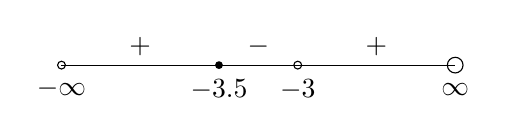
\begin{tikzpicture}	
			\draw
			(0,0) node[circle,draw,inner sep=1pt,label=below:$-\infty$](){}
		 -- (2,0) node[circle,fill,inner sep=1pt,label=below:$-3.5$](){} node[midway,above]{$+$}
		 -- (3,0) node[circle,draw,inner sep=1pt,label=below:$-3$](){} node[midway,above]{$-$}
		 -- (5,0) node[circle,draw,inner sep=2pt,label=below:$\infty$](){} node[midway,above]{$+$};
		\end{tikzpicture}
	\end{center}
	\[x\in\interval[open left, scaled]{-\infty}{-\frac72}\cup(-3,\infty)\]
\end{minipage}
\begin{minipage}[t]{0.49\linewidth}
	\begin{align*}
		\frac{1}{2(a+3)}&\leq1 \\
		\frac{1}{2(a+3)}-\frac{2(a+3)}{2(a+3)}&\leq0 \\
		\frac{-2a-5}{2a+6}&\geq0
	\end{align*}
	\begin{center}
		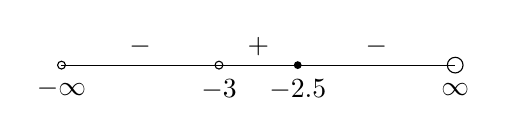
\begin{tikzpicture}	
			\draw
			(0,0) node[circle,draw,inner sep=1pt,label=below:$-\infty$](){}
		 -- (2,0) node[circle,draw,inner sep=1pt,label=below:$-3$](){} node[midway,above]{$-$}
		 -- (3,0) node[circle,fill,inner sep=1pt,label=below:$-2.5$](){} node[midway,above]{$+$}
		 -- (5,0) node[circle,draw,inner sep=2pt,label=below:$\infty$](){} node[midway,above]{$-$};
		\end{tikzpicture}
	\end{center}
	\[a\in(-\infty,-3)\cup\interval[open right, scaled]{-\frac52}{\infty}\]
\end{minipage}
\vspace*{10pt}

Notice that if $a=-3$, then $1/2(a+3)$ would be undefined, which means $\sin2c$ must be equal to it and thus $f$ would have no critical points.

\[a\in\paren{\interval[open left, scaled]{-\infty}{-\frac72}\cup(-3,\infty)}\cap\paren{(-\infty,-3)\cup\interval[open right, scaled]{-\frac52}{\infty}}\cup\{3\}\]
\begin{center}
	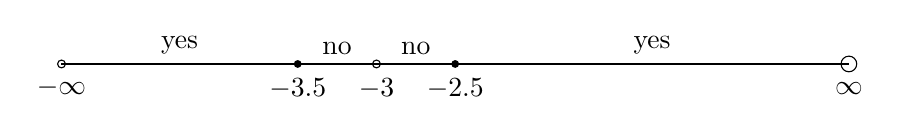
\begin{tikzpicture}	
		\draw
		(0,0) node[circle,draw,inner sep=1pt,label=below:$-\infty$](){}
	 -- (3,0) node[circle,fill,inner sep=1pt,label=below:$-3.5$](){} node[midway,above]{yes}
	 -- (4,0) node[circle,draw,inner sep=1pt,label=below:$-3$](){} node[midway,above]{no}
	 -- (5,0) node[circle,fill,inner sep=1pt,label=below:$-2.5$](){} node[midway,above]{no}
	 -- (10,0) node[circle,draw,inner sep=2pt,label=below:$\infty$](){} node[midway,above]{yes};
	\end{tikzpicture}
\end{center}
But, we want the values of $a$ that do not satisfy the inequality, so we take the intervals marked ``no.''

\begin{align*}
	a&\in\interval[open right, scaled]{-\frac72}{-3}\cup\interval[open left, scaled]{-3}{-\frac52}\cup\{3\} \\
	\Aboxed{a&\in\left[-\frac72,-\frac52\right]}
\end{align*}
This set does not contain $2$, which is good.

\end{document}
